% LaTeX/figure edition of the supplied working manuscript 0.1.
% Scientific source: docs/source/DCU_BRIDGES_MANUSCRIPT_v0_1.md.
% Compile from paper/: latexmk -lualatex -interaction=nonstopmode -halt-on-error main.tex
\documentclass[11pt,a4paper]{article}
\usepackage[margin=25mm,headheight=15pt]{geometry}
\usepackage{fontspec}
\setmainfont{Latin Modern Roman}
\setsansfont{Latin Modern Sans}
\setmonofont[Scale=MatchLowercase]{Latin Modern Mono}
\usepackage{amsmath,amssymb,amsthm,mathtools}
\usepackage{microtype}
\usepackage{graphicx,booktabs,longtable,array,calc}
\usepackage{caption}
\captionsetup{font=small,labelfont=bf,skip=7pt}
\usepackage{fancyhdr}
\usepackage{enumitem}
\usepackage{etoolbox}
\usepackage{url}
\usepackage{xurl}
\usepackage[hidelinks,unicode]{hyperref}
\usepackage[backend=biber,style=numeric,sorting=none,maxnames=3,giveninits=true,url=true,doi=true]{biblatex}
\addbibresource{references.bib}
\setlength{\bibitemsep}{4pt}
\renewcommand*{\bibfont}{\small}
\setlength{\emergencystretch}{2em}
\setlength{\parskip}{3pt}
\setlength{\parindent}{1em}
\setlength{\textfloatsep}{17pt plus 3pt minus 3pt}
\renewcommand{\topfraction}{0.88}
\renewcommand{\bottomfraction}{0.75}
\renewcommand{\textfraction}{0.10}
\renewcommand{\floatpagefraction}{0.72}
\setcounter{topnumber}{2}
\providecommand{\tightlist}{\setlength{\itemsep}{0pt}\setlength{\parskip}{0pt}}
\AtBeginEnvironment{longtable}{\small\setlength{\tabcolsep}{5pt}\renewcommand{\arraystretch}{1.14}}
\pagestyle{fancy}
\fancyhf{}
\fancyhead[L]{\small Registry structure and operational bridges}
\fancyhead[R]{\small J. Merwin}
\fancyfoot[C]{\thepage}
\renewcommand{\headrulewidth}{0.3pt}
\title{\vspace{-1.1em}\textbf{From Registry Structure to Physical Observables}\\[0.45em]\large Horizontal Transfers and Operational Bridges in the\\ Distinction Combinatorial Universe}
\author{Jason Merwin\\\small Independent Researcher}
\date{\small September 2026\quad\textbullet\quad Working manuscript 0.1, LaTeX edition}
\hypersetup{pdftitle={From Registry Structure to Physical Observables},pdfauthor={Jason Merwin},pdfsubject={Horizontal transfers and operational bridges in the DCU}}
\begin{document}
\maketitle
\thispagestyle{plain}
\begin{abstract}
The structural characterization of the 137-object distinction registry supplies a finite architecture but does not by itself identify physical particles or measurement operations. We investigate two routes from this architecture to observables. Horizontal transfers propagate fixed registry-based parameter prescriptions through explicitly borrowed physical laws; vertical bridges connect native construction and service histories to declared operational readouts. The horizontal examples include leptonic partial decay rates, recoil, reduced-mass spectroscopy, radiatively corrected pion branching, and neutrino propagation evaluated against published spectral information. The vertical results include workload back-action, shared-record clock covariance, history-dependent quantum channels, collective information protection, and measurement-induced disturbance. New information calculations identify the registry-overlap graph exactly with positive conditional mutual information between inherited record bundles after conditioning on their common genesis register. A finite-outcome inverse experiment estimates native service rates without revealing the hidden service histories to the estimator, while exposing reduced precision at low activity and non-identifiability of the separate queue and population. A separate audit distinguishes newly recorded Shannon information from construction workload. Successful transfers, insensitive comparisons, failed correspondences and missing physical identifications are retained separately. The study provides a quantitative map of the framework's current operational reach without assuming emergent three-dimensional space, identifying a neutron, or closing the remaining native mass and spacetime mappings.

\end{abstract}
\noindent\textbf{Keywords:} distinction registry; operational observables; parameter transfer; shared records; quantum channels; information; finite service.

\medskip
\noindent\begin{minipage}{\linewidth}\small\textit{Working-draft status.} This is a typeset and illustrated edition of the integrated first draft, not a submission-ready paper. No new bridge experiment is added here. The two proposed horizontal additions and final primary-reference reconciliation remain pending. Reproduction coverage is stated at the end of the paper and in the accompanying repository.\end{minipage}
\medskip
\section{Introduction}\label{introduction}

A structural theory becomes physically useful when its structures can be connected to observables by explicit rules that survive changes of apparatus, preparation or application. Numerical resemblance to a familiar constant is not sufficient, but requiring a complete account of space, matter and measurement before attempting any finite comparison is unnecessarily restrictive. Intermediate correspondences can be defined, computed and tested while their assumptions remain visible.

The preceding structural study characterizes the seven-vertex ancestry layer of the Distinction Combinatorial Universe (DCU). Its 137 objects have an inherited S/I/G classification of sizes 81, 40 and 16, and their overlap graph is exactly

\begin{equation}\label{eq:1}
\mathcal O=K_{11}\vee(K_{63}\sqcup K_{63}).
\end{equation}

The universal junction and two primitive-exchanged branches have compositions (9,2,0), (36,19,8), and (36,19,8). Full parentage distinguishes objects that the unweighted overlap graph cannot distinguish. The structural study also separates registry placement in constituent ancestry from placement in actual comparison-witness children. These are mathematical and computational results; their physical interpretation is a further problem \cite{D1}.

Here we investigate two complementary routes. A \textbf{horizontal transfer} takes a fixed registry-based parameter dictionary, an explicitly specified physical law, and any declared experimental inputs, and computes an observable not identical to the parameter itself. A \textbf{vertical bridge} starts from native structure or native activity and maps it to an operational measurement through a stated attachment. The first route tests the utility and limits of the parameter prescriptions. The second tests what actual DCU processes can support and what a specified observer could infer.

These routes are not yet a single closed derivation. In particular, a species-level proton mass prescription is not a function assigning a measured proton mass to an arbitrary native K3 motif. Likewise, a complex representation attached to native events is not a derivation of that representation from an unadorned counting process. Keeping these distinctions explicit allows substantial finite results without converting unresolved connections into implicit assumptions.

The aim is categorical: which bridges are quantitatively useful, which are operationally defined but not experimentally discriminated, which fail under their chosen correspondence, and which remain underdetermined? The negative and limiting results are part of that map, rather than reasons to redefine the successful cases.

\section{Definitions, source choices and evidence conventions}\label{definitions-source-choices-and-evidence-conventions}

\subsection{Native construction and service}\label{native-construction-and-service}

A composite object is an unordered pair \(z=\{u,v\}\) of distinct existing objects. A pair already present cannot be duplicated. A native state is ancestry-closed, and parentage is acyclic. The service process pools one maintenance request per object with outstanding recording obligations. If the population is \(n\), the outstanding work is \(F\), and the capacity is \(\Gamma\), then

\begin{equation}\label{eq:2}
R=F+n,\qquad q=\min(\Gamma,R).
\end{equation}

Exactly \(q\) requests are sampled uniformly without replacement. Every absent pair among the serviced maintenance objects is constructed; no selected favorable child is retained while other enabled children are suppressed. First-use and repeat recording charges differ, and the relief mechanism is a constitutive part of the specified process \cite[Section 2]{D2}.

For an old object \(z\), let \(\operatorname{Ch}(z)\) count primitive-rooted directed paths and let \(L_z=2\operatorname{Ch}(z)-2\). If \(h_z\) counts the events in a burst using its ancestry factor, the burst charge is

\begin{equation}\label{eq:3}
C=2\sum_z L_z h_z+9\sum_{z\in U}L_z\mathbf 1_{\{h_z>0\}},
\end{equation}

where \(U\) is the pre-burst unread set. The charged obligations and the requests actually serviced are different quantities. A native maintenance tick is one serviced maintenance request, not one service iteration and not an assigned interval in seconds.

The paper's capacity-two asymptotic theorems are not silently extended to the capacity-three experiments used here. The latter retain their exact finite sampler and full burst accounting.

\subsection{Record values and the quantum attachment}\label{record-values-and-the-quantum-attachment}

At its first write, each recorded composite receives an independent uniform trit \(g_z\in\{0,1,2\}\), retained on subsequent occurrences. An entry token \((z,e)\) reads \(s^e(g_z)\), where \(s=(0\;1)\) fixes 2. These values do not enter the present native counting transition \cite[Section 5]{D2}.

The finite quantum instrument additionally specifies a complex representation, source preparations, phase operations and Born readouts. Its two-factor shared source is

\begin{equation}\label{eq:4}
|\Omega\rangle=\frac{|00\rangle+|11\rangle+|22\rangle}{\sqrt3},
\end{equation}

under the source's stated diagonal-sector and common-character premises. A service-driven phase uses

\begin{equation}\label{eq:5}
D(x)=\operatorname{diag}(1,e^{2\pi ix},e^{4\pi ix}).
\end{equation}

The primary phase increment in the operational experiments is 1/27, with 1/81 retained as a specified finer-increment control. These are internal phase increments, not spatial dimensions or a change of units applied to the same increment. Count-driven phase retention and any fan-out to multiple readers are explicit attachments, not feedback laws already present in the constructor.

\subsection{Fixed dictionary and external inputs}\label{fixed-dictionary-and-external-inputs}

The executed horizontal branch uses the following exact prescriptions, with masses in electron-mass units:

\begin{table}[htbp]\centering
\caption{Frozen mass prescriptions used by the executed horizontal calculations. Entries are in electron-mass units.}\label{tab:dictionary}
\small\setlength{\tabcolsep}{5pt}\renewcommand{\arraystretch}{1.15}
\begin{tabular}{@{}lll@{}}

\toprule\noalign{}
Quantity & Screened prescription & Structural-only comparison \\
\midrule\noalign{}

Muon & \(827/4\) & \(411/2\) \\
Tau & \(13909/4\) & \(6987/2\) \\
Charged pion & \(273+20/137\) & \(273\) \\
Proton & \(1836+20/137\) & \(1836\) \\
Lambda & \(2183+45/137\) & \(2183\) \\
\bottomrule
\end{tabular}
\end{table}

These are the expressions actually used in the saved experiments. Some printed source papers use slightly different rounded lepton bases; they are not substituted into a completed calculation. The structural and screened recipes are distinct hypotheses, not interchangeable rounding conventions \cite{D3,D4,D5,R17,R18,R19,R20,R21,R22,R23}.

The neutrino branch retains

\begin{equation}\label{eq:6}
s_{12}=\sin^2\theta_{12}=\frac{167}{548},\qquad
s_{13}=\sin^2\theta_{13}=\frac{400}{18769},
\end{equation}

\begin{equation}\label{eq:7}
\Delta m_{21}^2=\frac{(m_ec^2)^2}{4\cdot137\cdot136^6},\quad
\Delta m_{32}^2=33\Delta m_{21}^2,\quad
\Delta m_{31}^2=34\Delta m_{21}^2.
\end{equation}

Dimensional comparisons borrow specified inputs, not an unreported universal calibration: the electron rest-energy unit for masses and kinematics; the muon lifetime for weak partial-rate normalization; the hydrogen 1S--2S interval for reduced-mass spectroscopy; measured electromagnetic coupling for the pion radiative correction; and a measured charged-kaon mass for associated-production channels whose dictionary base remains open. Neutrino spectrum comparisons additionally use the named experiments' flux, baseline, background, response or likelihood information.

\subsection{What counts as evidence}\label{what-counts-as-evidence}

We distinguish laboratory data, published parameter/likelihood summaries, deterministic forward predictions, exact model identities, and simulated measurement statistics. Related outputs sharing masses, data or calibrations are not independent confirmations. A favorable numerical residual is not a fitted theory-error allowance. A failure of a particular observable is not a proof that every possible correspondence fails.

The investigations are retrospective unless explicitly described as a newly fixed computational test. New synthetic estimates on fresh prepared states are not historically blind physical predictions. Statements concerning the late structural catalogue retain its incomplete service/queue audit scope.

\section{Horizontal transfers}\label{horizontal-transfers}

\subsection{Mass prescriptions into weak partial rates}\label{mass-prescriptions-into-weak-partial-rates}

The universal leading-order weak decay law, including final-lepton phase space, converts the fixed muon and tau mass ratios and one measured muon lifetime into tau electronic and muonic partial rates. The screened branch differs from the saved experimental partial-rate comparisons by approximately −0.31178\% and −0.36592\%, respectively; the structural-only comparison differs by about +5.18\% \cite{R17}.

These are partial rates. A total tau lifetime also requires its other channels, and the channel ratio is a dependent consequence rather than a third independent result. Radiative and finite-W corrections were not fitted or included in this experiment. The significance of the exercise is the successful transfer of one fixed prescription into two related rate observables under an explicit physical law, not emergence of the weak interaction from native recording work.

\begin{figure}[tbp]
\centering
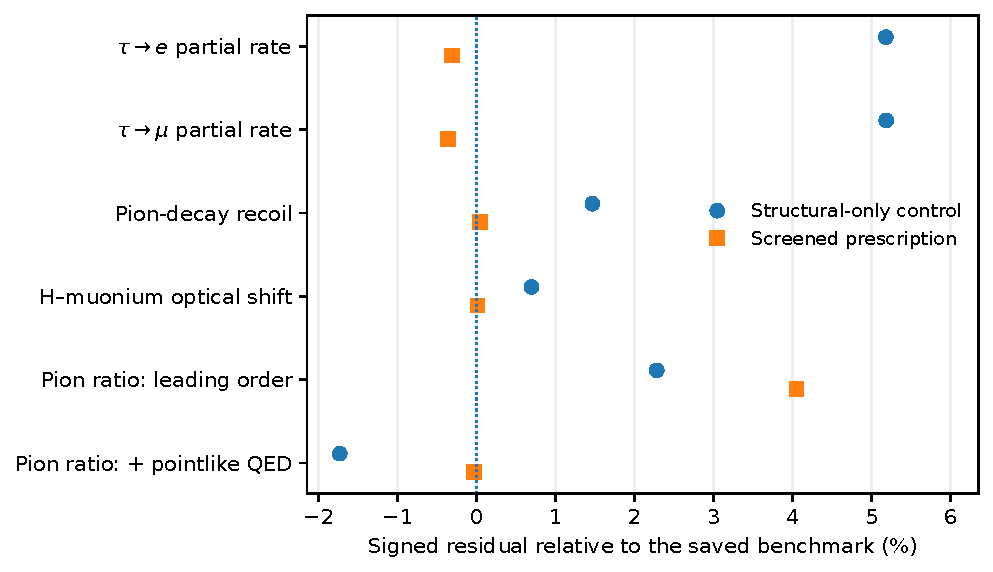
\includegraphics[width=0.97\linewidth]{figures/horizontal_residuals.pdf}
\caption{Signed residuals for the frozen structural-only and screened prescriptions, extracted from Cells 17--19. Rows share mass inputs and sometimes observations; they are not independent confirmations. The two pion-ratio rows differ in their borrowed radiative approximation. No common theoretical uncertainty or combined score is assigned.}\label{fig:horizontal}
\end{figure}

Figure \ref{fig:horizontal} compares these rate results with the subsequent recoil, optical, and pion-ratio transfers.

\subsection{Recoil and reduced-mass spectroscopy}\label{recoil-and-reduced-mass-spectroscopy}

Relativistic two-body conservation gives a screened pion-decay muon momentum of 29.804657018 MeV/c, approximately +0.0424846\% relative to the saved benchmark. The corresponding kinetic energy, neutrino energy and velocity are derived outputs of the same kinematics, not additional independent experimental tests \cite{R18}.

Reduced-mass scaling transfers the fixed ratios into the hydrogen--muonium 1S--2S difference, with a residual of approximately +0.0119670\%. The absolute muonium line and this difference are two presentations of one comparison. Differential bound-state QED, nuclear size, relativistic recoil and other omitted contributions are not absorbed into an empirical correction. These examples show useful quantitative reach, but do not establish that the same approximation remains precise arbitrarily close to thresholds or in every bound system.

\subsection{Diagnosing a missing physical term with a measured-input control}\label{diagnosing-a-missing-physical-term-with-a-measured-input-control}

The leading-order pion electronic/muonic branching calculation initially differs from the saved inclusive measurement by +4.049821\%. Substituting measured masses into the same leading-order formula gives a similar +4.108523\% difference. The shared discrepancy points to the common approximation rather than uniquely to the mass dictionary \cite{R18}.

A specified pointlike inclusive radiative term, recalculated from each mass recipe and measured electromagnetic coupling, changes the respective residuals to −0.037993\% and +0.018330\% \cite{R19}. It is not a fitted universal percentage and is not transferred to the effective weak mixing angle. Additional structure-dependent and resummed contributions remain outside the calculation.

This paired control provides a methodological result: a transfer can fail because its borrowed law is incomplete even when its parameter input is adequate at that accuracy. Conversely, the residual after adding one known correction does not establish a complete precision theory.

\subsection{Neutrino waveforms, detector folding and released spectral information}\label{neutrino-waveforms-detector-folding-and-released-spectral-information}

The fixed electron-row mixing weights and splittings determine the full coherent three-flavor vacuum survival function. Neither the atmospheric mixing angle nor the CP phase is required for this particular survival channel. Setting a common propagation eigenvalue to zero removes an unobservable phase; it does not determine the physical lightest mass \cite{R20}.

The exact integer splitting ratio produces a vacuum recurrence in the mathematical waveform. An approximate detector fold using the KamLAND 2005 release predicts 233.195 signal-plus-background candidates against 258 observed, with a fixed-nuisance Poisson deviance of 19.17383. The corresponding no-oscillation calculation gives 75.81426. These are diagnostics of the reconstruction, not the collaboration likelihood. Its baseline and energy averaging erase useful sensitivity to the exact fast-frequency integer; a visually plausible spectrum is therefore not confirmation of literal R=33 \cite{R21}.

The released Daya Bay 3158-day normal-ordering two-parameter surface provides a more direct atmospheric-frequency test. The unchanged predicted point gives \(\Delta\chi^2=0.514425153\) by primary bilinear interpolation, with a local cubic check of 0.506933978. Neighboring fixed alternatives R=32 and R=34 yield 1.644361118 and 2.694751797; none replaces the primary value \cite{R22}.

This establishes compatibility on the specified released surface under its solar priors and nuisance treatment. It is not a posterior probability of the framework, a complete four-parameter likelihood, or unique identification of an exact integer. The source inputs overlap historical global fits, so the associated comparisons are not counted independently.

\begin{figure}[tbp]
\centering
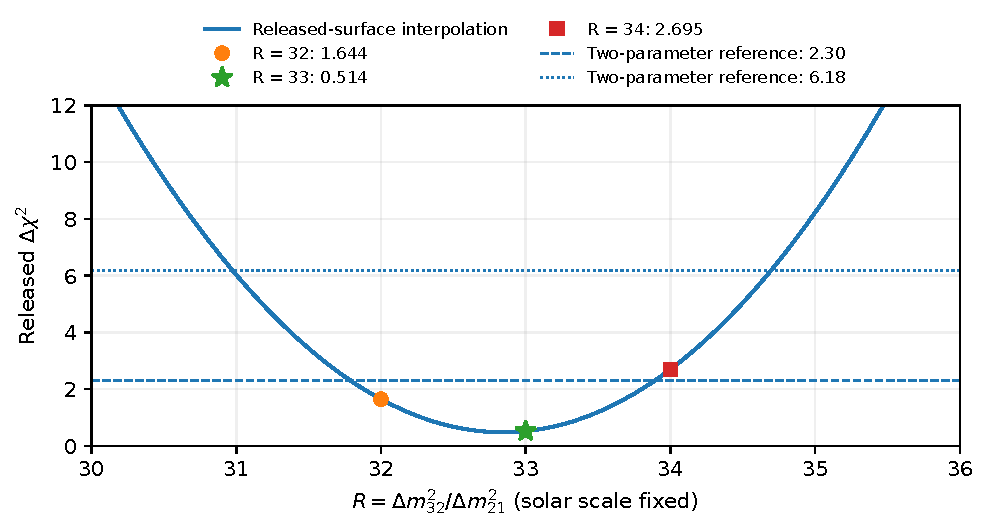
\includegraphics[width=0.96\linewidth]{figures/neutrino_profile.pdf}
\caption{The fixed-amplitude slice through the released Daya Bay 3158-day normal-ordering surface, using the unchanged source solar scale. Points mark the already declared R=32, 33 and 34 cases; R=33 remains primary. Dashed reference levels concern the original two-parameter surface, not a newly fitted one-parameter confidence interval or a probability of the theory. The collaboration solar and nuisance treatment is retained.}\label{fig:neutrino}
\end{figure}

Figure \ref{fig:neutrino} displays the frozen spectral-surface comparison.

\subsection{Thresholds, mixed sectors and the present boundary}\label{thresholds-mixed-sectors-and-the-present-boundary}

The same masses yield allowed invariant-mass boundaries and fixed-target thresholds under borrowed relativistic conservation. These values were compared with measured-mass control calculations, not independent production-onset data. A near-threshold velocity example shows how a small absolute mass discrepancy can become a large relative difference in a small kinetic quantity \cite{R23}. Production yields and angular rates require an interaction amplitude beyond kinematic permission.

The parameter-level angle ladder has mixed residuals and an atmospheric-octant dependence in the published comparison choices. Its effective weak angle is not interchangeable with another electroweak renormalization convention. The cosmological fraction comparison likewise does not supply Friedmann dynamics, a native density field or a new cosmological likelihood. These sectors remain in the complete evidence inventory without being promoted into stronger bridges than were calculated.

\section{Vertical bridges from native activity}\label{vertical-bridges-from-native-activity}

\subsection{Recording back-action and shared-record clock geometry}\label{recording-back-action-and-shared-record-clock-geometry}

A completed legal comparison can increase both outstanding recording work and population. In the controlled one-new-child comparison, the next tagged-token service probability changes by

\begin{equation}\label{eq:8}
\frac{p_{\mathrm{write}}}{p_{\mathrm{control}}}
=\frac{R_0}{R_0+C+1}.
\end{equation}

The charge is calculated from native ancestry and recorded status, not fitted to the subsequent slowdown. Longer continuations include changing graph, workload and relief. The immediate slowdown applies equally to old tokens; it is not a local gravitational lapse \cite{R25,R29}.

For maintenance indicators \(I_z\), let \(Y_A=\sum_{z\in A}I_z\), \(p=q/R\), and \(p_2=q(q-1)/[R(R-1)]\). Then

\begin{equation}\label{eq:9}
\operatorname{Cov}(Y_A,Y_B\mid Z)
=(p-p_2)|A\cap B|+(p_2-p^2)|A||B|.
\end{equation}

For equal-size supports, the common term cancels in the difference:

\begin{equation}\label{eq:10}
\operatorname{Var}(Y_A-Y_B\mid Z)
=(p-p_2)|A\triangle B|.
\end{equation}

A finite-horizon martingale identity relates accumulated difference variance to integrated activity. This gives an operational support metric and a clock-only reference normalization. The identity applies to general fixed subsets under exchangeable sampling; its validity does not by itself require the 81/40/16 sectors. Different entry paths with identical register sets remain indistinguishable to this support-only clock \cite{R26}.

\subsection{A full native-history quantum channel}\label{a-full-native-history-quantum-channel}

The joint distribution of two tagged service counts defines

\begin{equation}\label{eq:11}
\mathcal E(\rho)=\sum_{a,b}p_{ab}
[D(a/Q)\otimes D(b/Q)]\rho[D(a/Q)\otimes D(b/Q)]^\dagger.
\end{equation}

This is a completely positive trace-preserving map because it is a probability mixture of unitary conjugations. Its history dependence comes from native service and workload, while its complex phases and quantum source are inherited instrument assumptions. Classical sampling does not generate the initial entanglement \cite{R32}.

For the diagonal shared source, the sum \(K=a+b\) is sufficient. Two characteristic moments,

\begin{equation}\label{eq:12}
C_h=\mathbb E e^{2\pi i hK/Q},\qquad h=1,2,
\end{equation}

determine the density matrix and its negativity,

\begin{equation}\label{eq:13}
\mathcal N=\frac{2|C_1|+|C_2|}{3}.
\end{equation}

A source-backed filtered preparation transfers through the same full channel, but no longer permits the sum-only compression. Thus the transfer both validates the richer operational description within the model and locates a specific loss of information in the reduced description.

At a fixed later readout, the signed Bell witness can lose its violation while negativity remains positive. Known-history phase inversion restores the original state, whereas phase averaging generally reduces coherence. These distinguish a failed fixed witness, uncertain phases and separability; they are not interchangeable descriptions of collapse.

\subsection{Interventions and persistence}\label{interventions-and-persistence}

A fixed ideal echo exchanges basis labels 0 and 2 at the midpoint and at the final readout. Its exact action replaces early-plus-late phase accumulation by early-minus-late accumulation, up to a global phase. At the primary 1/27 increment it improves fidelity without restoring the terminal fixed Bell violation. At the retained 1/81 control it restores that violation in all six saved ensembles. Negativity does not improve uniformly \cite{R33}.

The intervention depends on correlations between windows, not merely separate marginal channels. A finite counterexample supplies two histories with identical free channels at both checkpoints but different echo responses. The control therefore tests information not contained in either free channel separately. Its scheduling and resource cost remain ideal additions.

A later-epoch study selects native paths through 4,194,304 maintenance ticks. For a fixed early-selected pair, late preparation greatly improves retention over 8,192 global maintenance ticks but gives no detected improvement after the same 32 services to the actual support. The large change in global longevity is explained by reduced local exposure \cite{R35}.

Collective incidence identities provide a separate positive result. Four actual paths satisfying

\begin{equation}\label{eq:14}
\mathbf1_A+\mathbf1_B=\mathbf1_C+\mathbf1_D
\end{equation}

protect the readable code \(\operatorname{span}\{|00\rangle,|11\rangle,|22\rangle\}\) under an explicit aggregate-input attachment. Some identities also balance entry tokens. This is exact protection against the specified common driving operations, not a binding energy or an autonomous particle.

\begin{figure}[tbp]
\centering
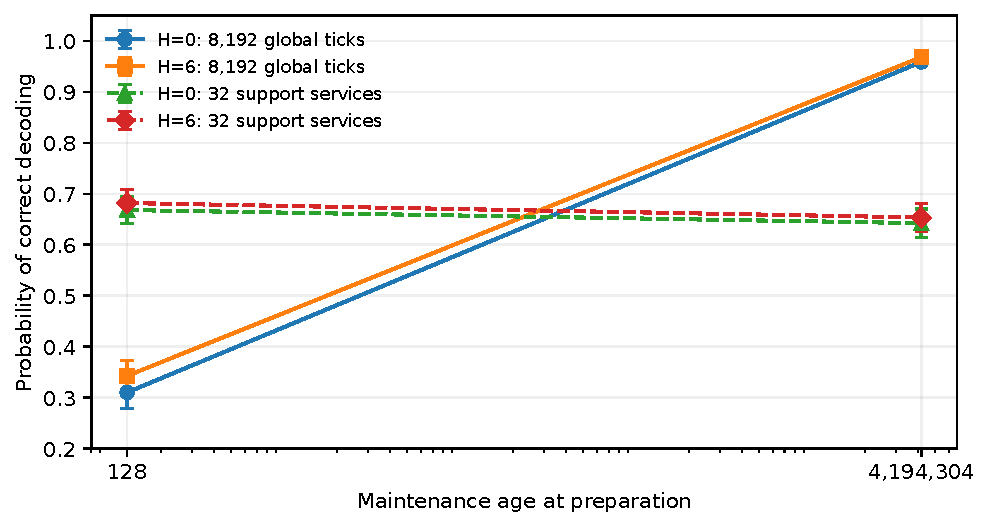
\includegraphics[width=0.95\linewidth]{figures/epoch_activity.pdf}
\caption{Activity-matched persistence of the same early-selected record pair in early and late native states (Cell 35). The phase increment is 1/27. Error bars are sample standard errors for 128 expected readouts in each regime/age/window, conditional on four source worlds. Lines connect the two measured preparation ages only. Global-tick longevity improves while retention after matched support activity does not show the same gain.}\label{fig:epoch}
\end{figure}

Figure \ref{fig:epoch} contrasts the global-age and local-activity observation windows.

\section{New information and inverse-measurement bridges}\label{new-information-and-inverse-measurement-bridges}

\subsection{Shared native records as Shannon information}\label{shared-native-records-as-shannon-information}

Let \(Y_A\) denote the full ordered readout of a structurally selected path with register set \(A\) and fixed entry conventions. Conditioning on its graph, each distinct register supplies one independent uniform trit, and the entry map is invertible. Consequently,

\begin{equation}\label{eq:15}
H(Y_A)=|A|\log_2 3,
\qquad
H(Y_A,Y_B)=|A\cup B|\log_2 3,
\end{equation}

\begin{equation}\label{eq:16}
I(Y_A;Y_B)=|A\cap B|\log_2 3,
\end{equation}

\begin{equation}\label{eq:17}
I(Y_A;Y_B\mid Y_C)=|(A\cap B)\setminus C|\log_2 3.
\end{equation}

These are consequences of the inherited first-write model and Shannon's entropy definition \cite{E1}, not new dynamics. The conditional formula follows by substituting the corresponding union cardinalities into the four-entropy identity. Conditioning on a third reader can remove shared information by revealing the common registers; this is not a causal or gravitational screening claim.

All 1,913 pairs from the 116 archived three- and four-register paths were checked by complete distribution enumeration. Forty-six structurally selected triple cases were also enumerated. Independent finite-field rank calculations reproduce the results because the reflection is the affine map 1−g modulo three \cite{R38}.

A prefix-only readout loses information. Equal-support paths entering a shared register from opposite sides can carry full mutual information even though their literal addresses agree with probability only one third. Symbol equality therefore cannot substitute for shared information when the readout frames are known.

Finite sampling preserves an important limitation. For the four H0 length-three representatives at 65,536 independent register-value realizations, the exact mutual informations 0, 1.5849625, 3.1699250 and 4.7548875 bits give plug-in estimates 0.0082585, 1.5872795, 3.1702006 and 4.7546720. The nonzero disjoint estimate is sampling bias, not a physical interaction. The samples are independently prepared first-write valuations of a fixed graph, not new draws on every maintenance tick of one persistent world.

\begin{figure}[tbp]
\centering
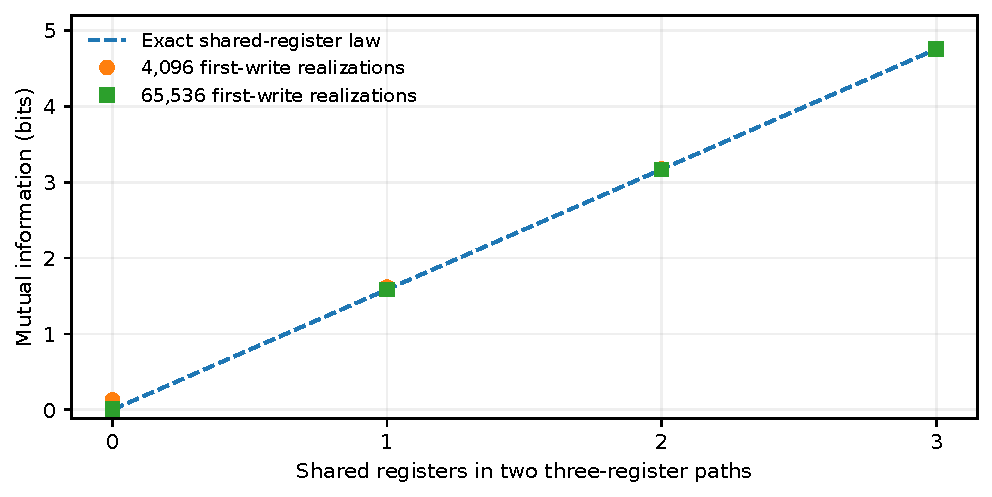
\includegraphics[width=0.95\linewidth]{figures/record_information.pdf}
\caption{Mutual information of the four frozen H0 three-register representatives (Cell 38). Each sample is an independent first-write valuation at a fixed graph, not a new trit drawn at every maintenance service. All four shared-register classes are retained. The positive plug-in estimate at zero shared registers is finite-sample bias; the exact model value is zero.}\label{fig:information}
\end{figure}

Figure \ref{fig:information} retains the exact sharing law and its finite-sample estimates.

\subsection{The registry as a conditional-information graph}\label{the-registry-as-a-conditional-information-graph}

The complete size-bounded registry ideal contains 173 objects, of which 137 have inclusive ancestry size seven. For a registry root \(r_i\), define

\begin{equation}\label{eq:18}
B_i=\operatorname{Anc}(r_i)\setminus\{a,b,r_i\}.
\end{equation}

Each \(B_i\) contains four proper nonprimitive ancestors. Their registers are already recorded because each has a child on a path to \(r_i\). The root's own possibly unread register and the two primitives are not treated as available random trits. Let \(Y_i\) be the complete ordered bundle of these four ancestral values. This is an explicit multi-record observation convention, not a claim that every root autonomously reads its full ancestry.

Every registry root contains the genesis composite \(c=\{a,b\}\). Distinct roots of the same ancestry size cannot be ancestors of one another. Hence

\begin{equation}\label{eq:19}
\boxed{
I(Y_i;Y_j\mid g_c)
=\bigl(|\operatorname{Anc}(r_i)\cap\operatorname{Anc}(r_j)|-3\bigr)\log_2 3.
}
\end{equation}

The existing overlap threshold of more than three common ancestors is therefore exactly positivity of conditional mutual information after the shared genesis record is known. All 9,316 root-pair distributions were checked:

\begin{table}[htbp]\centering
\caption{Exact registry-pair distribution after conditioning on the common genesis register.}\label{tab:registry_pairs}
\small\setlength{\tabcolsep}{5pt}\renewcommand{\arraystretch}{1.15}
\begin{tabular}{@{}rr@{}}

\toprule\noalign{}
Conditional shared trits & Pair count \\
\midrule\noalign{}

0 & 3,969 \\
1 & 3,774 \\
2 & 1,323 \\
3 & 250 \\
\bottomrule
\end{tabular}
\end{table}

The positive-information graph has 5,347 edges and recovers the exact junction/two-branch form of D1. Each full branch bundle contains 17 distinct ancestral registers; their only shared register is c, so the two whole bundles are conditionally independent given g\_c under this first-write model \cite{R38}.

This supplies a quantitative information interpretation of the registry architecture without spatial coordinates. It is not independent evidence that 137 is physically necessary: the information graph is induced by the already established overlaps and the declared independent-register model. Nor does conditional independence imply absence of native future contact.

The measurement also has a finite resolution limit. There are only 37 distinct proper-register bundles among the 137 roots: 25 occur for five roots each and 12 occur once. Final parent-pair distinctions can therefore remain invisible even to the complete ancestral-value bundle. The S/I/G classification still requires the inherited full structural rule; the information graph does not independently recover all sector identities. In particular, every individual four-trit marginal is uniform, and joint correlations---not a single isolated outcome---carry the graph information.

\begin{figure}[tbp]
\centering
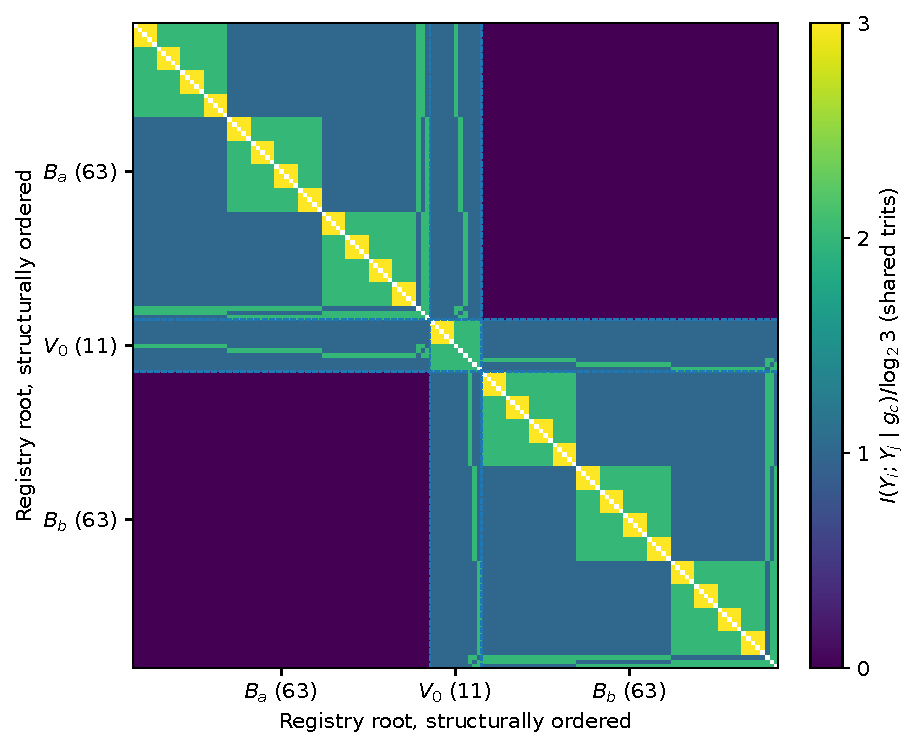
\includegraphics[width=0.83\linewidth]{figures/registry_information.pdf}
\caption{The exact conditional-information matrix for all distinct pairs of registry roots, in units of shared trits. Roots are ordered by the inherited branch--junction--branch decomposition, not by fitted clustering. The diagonal is excluded. Positive entries recover the 5,347-edge overlap graph; the two 63-root branches share no remaining information after conditioning on the genesis register. This is a dependence structure of the declared record variables, not a spatial map or an independent derivation of sector identities.}\label{fig:registry}
\end{figure}

Figure \ref{fig:registry} displays the complete pairwise conditional-information table.

\subsection{Inferring native activity without exposing hidden counts}\label{inferring-native-activity-without-exposing-hidden-counts}

The previous vertical studies mostly evaluated observables from known native histories. We now reverse that direction once. At a fixed capacity-three pre-service state, the total increment \(K\) of two tagged maintenance tokens has law

\begin{equation}\label{eq:20}
(w_0,w_1,w_2)=(1-2p+p_2,\;2(p-p_2),\;p_2),
\end{equation}

\begin{equation}\label{eq:21}
p=\frac3R,\qquad p_2=\frac6{R(R-1)}=\frac{2p^2}{3-p}.
\end{equation}

Use the inherited difference-outcome kernel at nine fixed offsets x=j/9:

\begin{equation}\label{eq:22}
P(s\mid K,x)=\frac{[1+2\cos(2\pi(x+K/Q-s/3))]^2}{9}.
\end{equation}

The 27-by-3 mixture matrix has full column rank. The offset harmonics reveal C0,C1,C2, and their K=0,1,2 coefficients form a nonsingular Vandermonde matrix for Q=27 or 81. Thus the exact mixture is identifiable. For finite outcomes, the estimator uses the specified one-parameter native law and maximizes likelihood over the rate p.~It receives only outcome counts, fixed settings and the apparatus model, never R, F, n, K, the state label or the service trajectory \cite{R39}.

Two fresh native trajectories, H=0 and H=6, supply all six states at iterations 16,64,256 after the unchanged five-object source preparation. The preparation's 26 work obligations and five maintenance ticks are retained. These are dependent checkpoints of two trajectories, not six independent universes. For each state and phase increment, 64 synthetic measurement datasets use 32,768 ideal independent shots per offset. Multinomial counts sample the exact one-step outcome law; a full native growth history is not simulated for every shot.

\begin{table}[htbp]\centering
\caption{Finite-outcome activity estimates for all six new prepared states. Relative RMSE is computed across 64 synthetic datasets per state at the primary phase increment.}\label{tab:inverse}
\small\setlength{\tabcolsep}{5pt}\renewcommand{\arraystretch}{1.15}
\begin{tabular}{@{}lrrrr@{}}
\toprule State & True $R$ & True $p$ & Median $\widehat p$ & Relative RMSE \\\midrule
H0, iteration 16 & 39 & 0.0769231 & 0.077150 & 2.88\% \\
H0, iteration 64 & 51 & 0.0588235 & 0.058973 & 3.66\% \\
H0, iteration 256 & 261 & 0.0114943 & 0.011749 & 10.46\% \\
H6, iteration 16 & 9 & 0.3333333 & 0.333313 & 0.76\% \\
H6, iteration 64 & 150 & 0.0200000 & 0.019712 & 7.62\% \\
H6, iteration 256 & 385 & 0.0077922 & 0.007968 & 11.90\% \\
\bottomrule
\end{tabular}
\end{table}

The finer-increment control has worse precision, reaching 39.60\% relative RMSE at the least active state. The apparatus matrices' condition numbers are approximately 65.5 and 595.9. These demonstrate the distinction between exact identifiability and finite-shot sensitivity; neither the increment nor the shot budget was changed to obtain a desired accuracy.

Only \(R=F+n\) is identified. Different valid native states with the same R have the same law in this experiment, so F and n separately remain unresolved without additional information. Recovery is conditional on the assumed sampler and measurement family; it does not independently validate that sampler or establish a physical clock rate in seconds. Repreparation, global service-step timing and access to the readout remain ideal resources rather than an autonomous native observer.

\begin{figure}[tbp]
\centering
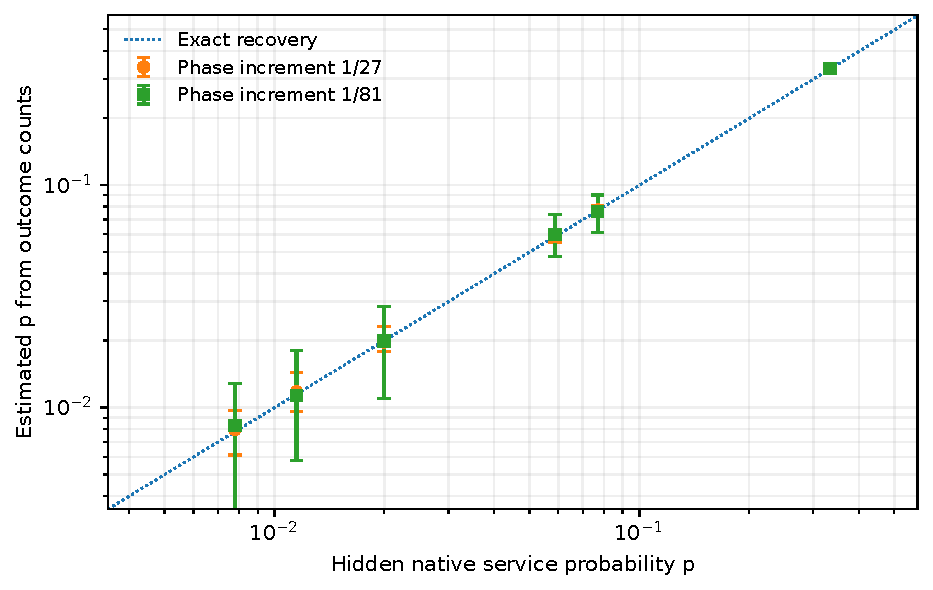
\includegraphics[width=0.91\linewidth]{figures/inverse_activity.pdf}
\caption{Recovery of the hidden native service probability from finite synthetic outcome counts (Cell 39). Markers are medians; bars show empirical central 95-percent ranges across 64 datasets at each of six new prepared states. They are not confidence intervals from a single measurement. Each dataset contains 32,768 ideal shots at each of nine settings. The smaller phase increment worsens sensitivity at the same shot budget.}\label{fig:inverse}
\end{figure}

Figure \ref{fig:inverse} shows the finite-outcome recovery and its sampling spread.

\subsection{Recording workload and information are not interchangeable}\label{recording-workload-and-information-are-not-interchangeable}

A secondary audit uses all 21 productive events in the same 512 new native preparation steps. If \(W_{\mathrm{new}}\) is the set of first-written nonprimitive registers, then, conditional on the event history and old recorded values,

\begin{equation}\label{eq:23}
H(g_{W_{\mathrm{new}}}\mid g_{\mathrm{old}},\text{native event})
=|W_{\mathrm{new}}|\log_2 3.
\end{equation}

This is the entropy in newly written register values, available to a reader given access to those values. It excludes information in the choice of event, timing and the fuller record-factor algebra. The native work remains the ancestry-factor charge defined in Section 2.1.

\begin{table}[htbp]\centering
\caption{All productive events in the new continuation windows, grouped by new trit count.}\label{tab:work}
\small\setlength{\tabcolsep}{5pt}\renewcommand{\arraystretch}{1.15}
\begin{tabular}{@{}rrr@{}}

\toprule\noalign{}
New trits & Productive events & Native recording charge \\
\midrule\noalign{}

0 & 3 & 12--68 \\
1 & 17 & 48--408 \\
2 & 1 & 144 \\
\bottomrule
\end{tabular}
\end{table}

The same new trit information can require different native work, and repeat-only construction can cost work while writing no new trit. This is expected when one inventory counts retained register values and the other counts ancestry path factors and repeated uses. A universal proportionality between this Shannon-information increment and construction charge fails on the explicit finite examples. A thermodynamic energy or erasure interpretation would require additional definitions; neither temperature nor heat is inferred from these counts \cite{R39}.

\begin{figure}[tbp]
\centering
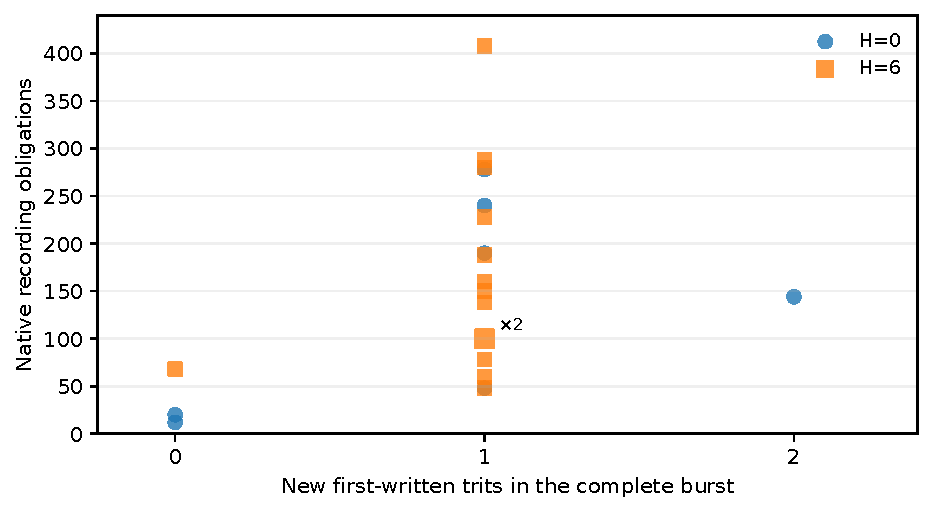
\includegraphics[width=0.91\linewidth]{figures/work_information.pdf}
\caption{Native recording obligations versus newly written trits for all 21 productive events in the two new continuation windows. Marker area reflects coincident event multiplicity within each regime, with repeated coordinates explicitly annotated. Equal trit increments can incur different work, and positive work can occur without a new trit. No temperature, heat or energy unit is assigned.}\label{fig:work}
\end{figure}

Figure \ref{fig:work} keeps all productive events in this work--information comparison.

\section{Implementation and identification boundaries}\label{implementation-and-identification-boundaries}

Readable information is not automatically preserved by reading. Separate local Fourier measurements and a coherent joint-label measurement can report identical label probabilities while leaving different states. Under the tested factor-local grammar without an additional shared quantum resource, perfect identification of the three encoded phase words leaves original-carrier fidelity at most one third. An explicit fresh-source renewal procedure reproduces the desired logical measurement on the protected code, but changes the carrier and is not equivalent outside that code \cite{R36,R37}.

Native bursts can create the replacement sibling resource and incur exactly calculated recording obligations. This does not account for every query, classical outcome record, conditional phase operation or reassignment of the storage driver. Those costs are unspecified, not zero. A correct ideal quantum transformation and a legal native construction are not, together, proof that the constructor implements the transformation.

Likewise, finite graph spectra do not uniquely select an energy operator. Signed and spectral-magnitude conventions can produce different cavity gaps on the same eigenvectors. The phase-only channel preserves populations in its chosen basis and hence cannot supply a diagonal-energy shift by itself. Exchangeable single-token clocks retain equal conditional mean service probabilities even when an external tracker changes their carrier labels. These results delimit the specific tested correspondences; they are not general prohibitions on additional DCU dynamics \cite{R23,R30,R31,R32,R33,R34,R35,R36,R37}.

The original fixed-reference K3 warmed-Q ratio screen found no neutron-sized positive excess among 467 occurrences. A separately defined contained-K3 attachment search found two local-excess leads with approximately 2.7--2.8\% errors relative to the small splitting. Their target-selected status, formation histories, virtual warmed preparation and different denominators remain explicit. They are exploratory structural-work leads, not particle identifications. Append-only historical persistence and a static warmed-Q value are not decay predicates \cite{N1,N2}.

No result in the present paper requires concluding that the neutron is absent, or waiting until one is identified. Similarly, the absence of a demonstrated three-dimensional physical manifold does not prevent finite information, service-rate or quantum-instrument measurements. It limits spatial propagation, physical localization and related valuations that require more than the present inputs.

\section{Categorical reach and conclusion}\label{categorical-reach-and-conclusion}

\begin{table}[htbp]\centering
\caption{Categorical reach of the executed bridges and the limits of each correspondence.}\label{tab:reach}
\small\setlength{\tabcolsep}{5pt}\renewcommand{\arraystretch}{1.15}
\begin{tabular}{@{}
  >{\raggedright\arraybackslash}p{(\columnwidth - 4\tabcolsep) * \real{0.3333}}
  >{\raggedright\arraybackslash}p{(\columnwidth - 4\tabcolsep) * \real{0.3333}}
  >{\raggedright\arraybackslash}p{(\columnwidth - 4\tabcolsep) * \real{0.3333}}@{}}

\toprule\noalign{}
\begin{minipage}[b]{\linewidth}\raggedright
Domain
\end{minipage} & \begin{minipage}[b]{\linewidth}\raggedright
Demonstrated reach
\end{minipage} & \begin{minipage}[b]{\linewidth}\raggedright
Present boundary
\end{minipage} \\
\midrule\noalign{}

Registry dictionary to physical observables & Quantitative rate, recoil, optical and oscillation transfers & Borrowed interactions, calibrations and data dependencies \\
Native work to activity & Exact conditional service response and finite continuations & Not local gravitational proper time \\
Shared ancestry to measurement correlations & Clock covariance, record entropy and conditional information & Readout aliases; not spatial distance \\
Registry to information organization & Exact conditional-information realization of the junction/two-branch graph & Does not distinguish all roots or derive sector identity from adjacency alone \\
Native activity to measured outcomes and back & A full quantum channel and finite-shot rate estimation & Ideal instrument/repreparation; only identifiable parameter combinations recovered \\
Persistence and interventions & Collective phase protection, echo response, activity-matched tests & No binding-energy or autonomous-particle identification \\
Recording to information accounting & Exact charge/record-entropy comparison & No universal bits-to-work conversion or thermodynamic valuation \\
Native mass, decay and spacetime & Explicit hypotheses and scoped negative results & Required active-state, energy, charge and spatial mappings remain distinct \\
\bottomrule
\end{tabular}
\end{table}

The contribution is the reuse of fixed descriptions across different observable questions. Horizontal success does not close the native particle mapping, and a native operational identity is not an independent laboratory confirmation. Nevertheless, the joint programme has advanced beyond either a bare structural census or a list of constants: it now includes conditional mechanisms, transferred preparations, controlled interventions, finite-outcome inversion and explicit non-identifiability results.

The registry's detailed architecture has an exact information interpretation, while more general ancestry and service principles explain other results. Identifying these different dependencies is essential. Future work can target the remaining maps without having to reopen every successful finite calculation. The present paper can therefore be completed as a bounded account of quantitative and operational reach, independently of a complete theory of particle identity or emergent spacetime.

\section{Reproducibility and verification scope}\label{reproducibility-and-verification-scope}

The historical horizontal and vertical sections summarize their saved versioned cells, results and notes. They have not all been rerun during this manuscript assembly. New Cells 38 and 39 are self-contained NumPy/Python files with embedded or generated small fixtures and plain JSON outputs.

The new information calculations enumerate 11,229 pair distributions across the record panels and registry, plus 46 conditional triple distributions. An independent validator uses finite-field rank calculations and an independent bitmask registry enumeration. The new service states are replayed against the original native constructor and Cell25 step for all 512 updates. All 896 inverse estimates are checked with an independently assembled density-matrix readout and separate optimizer. Numerical agreement is an implementation check, not physical precision. Finite-sample information bias and rate uncertainty remain in the complete results.

Large late-history structural certificates do not substitute for their unfinished queue and random-state audits. The main small-state operational results do not depend on reconstructing the entire late corpus. All counting/phase assumptions, counterfactual preparations and unknown implementation costs must accompany the released figures and tables.

\section{Distribution and outstanding work}\label{distribution-and-outstanding-work}

This LaTeX edition preserves the scientific results of working draft 0.1. Figures are generated directly from the frozen numerical files; the original Markdown remains in the repository. The compact reproduction command regenerates the horizontal Cells 14 and 17--24, re-evaluates Cells 32--34 from archived histories, executes the instrument calculations in Cells 36--37, reruns the new Cells 38--39, and checks the saved-record analysis of Cell 35. Exact rational fields and discrete records are checked separately from floating-point tolerances. The earlier native-history suite and the million-tick epoch generator are separate opt-in routes. The late neutron-search corpus is not reproduced by this distribution.

The two bounded horizontal additions---pointlike electromagnetic production and beta-endpoint effective mass---remain proposed rather than executed. The historical comparisons keep their original releases and conventions. Final primary-reference reconciliation and author review remain prerequisites for submission; this typeset edition does not convert those pending tasks into completed results.

\printbibliography[title={References and archived evidence}]
\end{document}
